\chapter{ER Diagram}

\section{實體與關係總覽}

\begin{figure*}[ht]
    \centering
    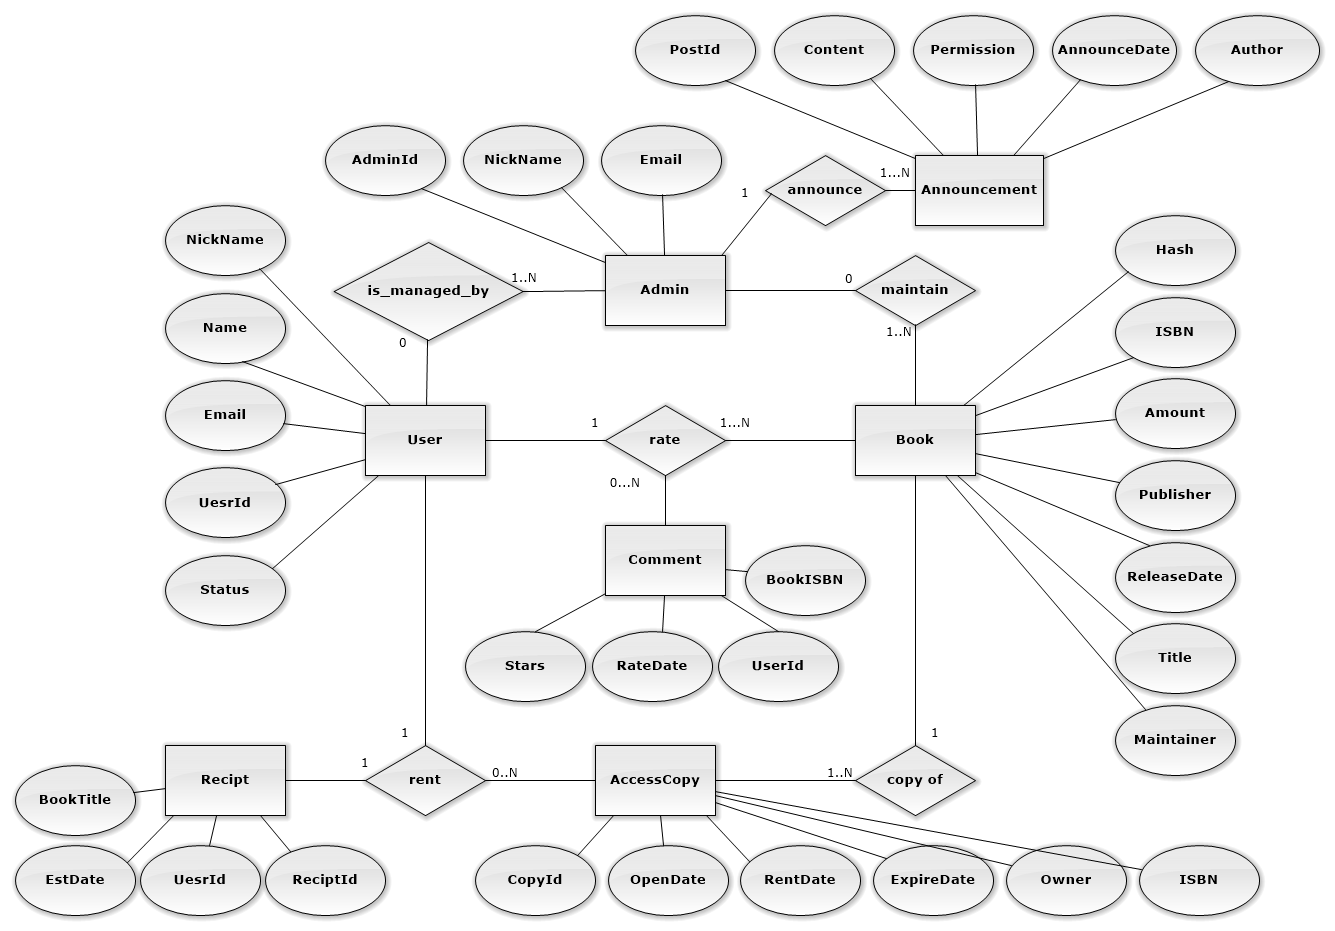
\includegraphics[width=\linewidth]{image/ChenERDiagram.png}
    \captionsetup{justification=centering}
    \caption{Chen ER Diagram}
\end{figure*}

\hspace*{-2em}User:

\begin{enumerate}
\item 屬性
    \begin{itemize}
    \item UserId(\textbf{主鍵};使用者ID)
    \item Name(姓名)
    \item Email(電子郵件)
    \end{itemize}
\item 關聯
    \begin{itemize}
    \item is\_managed\_by:使用者被零或一位管理員管理
    \item rent:使用者借閱零至多份副本(AccessCopy)
    \item read:使用者可閱讀零至多份副本(AccessCopy)
    \end{itemize}
\end{enumerate}

\hspace*{-2em}Admin:

\begin{enumerate}
\item 屬性
    \begin{itemize}
    \item AdminId(\textbf{主鍵};管理員ID)
    \end{itemize}
\item 關聯
    \begin{itemize}
    \item is\_managed\_by:管理員管理一至多位使用者
    \item maintain:管理員管理一至多本書籍
    \end{itemize}
\end{enumerate}

\hspace*{-2em}Book:

\begin{enumerate}
\item 屬性
    \begin{itemize}
    \item BookId(\textbf{主鍵};書籍ID)
    \item ISBN(書籍ISBN)
    \item Amount(正本數量)
    \item Publisher(出版社)
    \item ReleaseDate(出版日期)
    \end{itemize}
\item 關聯
    \begin{itemize}
    \item maintain:書籍管理零個管理員
    \item copy of:書籍可被複製成一至多份副本(AccessCopy),並具備時間戳記
    \item contain:書籍包含一至多個標題(Title)
    \end{itemize}
\end{enumerate}

\hspace*{-2em}Title:

\begin{enumerate}
\item 屬性
    \begin{itemize}
    \item TitleId(\textbf{主鍵};標題ID)
    \item BookId(\textbf{外鍵};連結到 Book 資料表)
    \item Language(標題語言)
    \item Title(標題文字)
    \end{itemize}
\item 關聯
    \begin{itemize}
    \item contain:標題包含一個書籍
    \end{itemize}
\end{enumerate}

\hspace*{-2em}AccessCopy:

\begin{enumerate}
\item 屬性
    \begin{itemize}
    \item CopyId(\textbf{主鍵};副本ID)
    \item OpenDate(借閱日期)
    \item ExpireDate(逾期日期)
    \item UserId(擁有者)
    \end{itemize}
\item 關聯
    \begin{itemize}
    \item read:副本被一位使用者閱讀
    \item copy of:副本對應一本原始書籍(Book)
    \end{itemize}
\end{enumerate}
  


\section{關係關聯說明}

\begin{enumerate}
    \item 「User」與「Admin」有一對多 (1..N) 管理關係(is\_managed\_by):  
      一位使用者可以被零或一位管理員管理(0..1),而一位管理員可以管理一至多位使用者(1..N)。
    \item 「User」與「AccessCopy」有一對多 (0..N) 借閱關係(rent):  
      一位使用者可以借閱零至多份副本(0..N),而每一份副本只能被一位使用者借出(1)。
    \item 「User」與「AccessCopy」有一對多 (0..N) 閱讀關係(read):  
      一位使用者可以閱讀零至多份副本(0..N),而每份副本只能被一位使用者閱讀(1)。
    \item 「Admin」與「Book」有一對多 (1..N) 管理關係(maintain):  
      一位管理員可以管理一至多本書(1..N),而一本書可以沒有管理員維護(0)。
    \item 「AccessCopy」與「Book」有一對多 (0..N) 來源關係(copy of):  
      一本書可以被複製成零至多份副本(0..N),而每份副本只能對應一本書籍(1),並記錄複製時間戳記。
    \item 「Book」與「Title」有一對多 (0..N) 書名關係(contain):  
      一本書可以有多個不同翻譯的書名(0..N),而每個標題只有對應一本書(1)。
  \end{enumerate}
  